%% ==============================================
%%               Use Cases
%% ==============================================
%% Author: Fabian Sorn
%% ==============================================

\chapter{Use Cases}
\label{ch:usecases}

This chapter will give an overview over different Use Cases that we will later use for the evaluation of the Plotting Libraries. All of these are different scenarios from Teams at CERN, that are looking into PyQt as an option to implement different \gls{gui} applications and need plots in their applications.




%% ==============================================
%%               BE-CO-HT
%% ==============================================
\section{Digital Oscilloscope for BE-CO-HT}
\label{sec:usecases:becoht}

The first Use Case we will investigate is coming from the \gls{ht}, who are planning to implement a \gls{gui} application showing a digital oscilloscope. For this they are interested in displaying a Line Graph in their application, which is showing up to eight curves with up to 100.000 points per curve. The goal for this graph would be an update rate of 25 updates per second.




%% ==============================================
%%               BE-OP-LHC
%% ==============================================
\section{Line Charts in section BE-OP-LHC}
\label{sec:usecases:becolhc}

The second Use Case we will investigate is coming from the \gls{lhcop}, who are interested in displaying a Line Graph containing 3000 datasets displayed as curves, who each will contain 2 * 3600 points. The data will be updated every second.


%% ==============================================
%%               BE-CO-APS
%% ==============================================
\section{Use case in Linac 4 Source GUI}
\label{sec:usecases:linac}

The third Use Case we wil investigate is coming from \gls{aps}. For this, multiple ScatterPlots should be displayed. The \gls{gui} Application will contain 4 different scatter plots, each containing up to 3 data sets, which each contain 1 hour of live data, which receives a new point roughly every 1.2 seconds. This results in 3000 visible points per data set.

\begin{figure}[h]
    \centering
    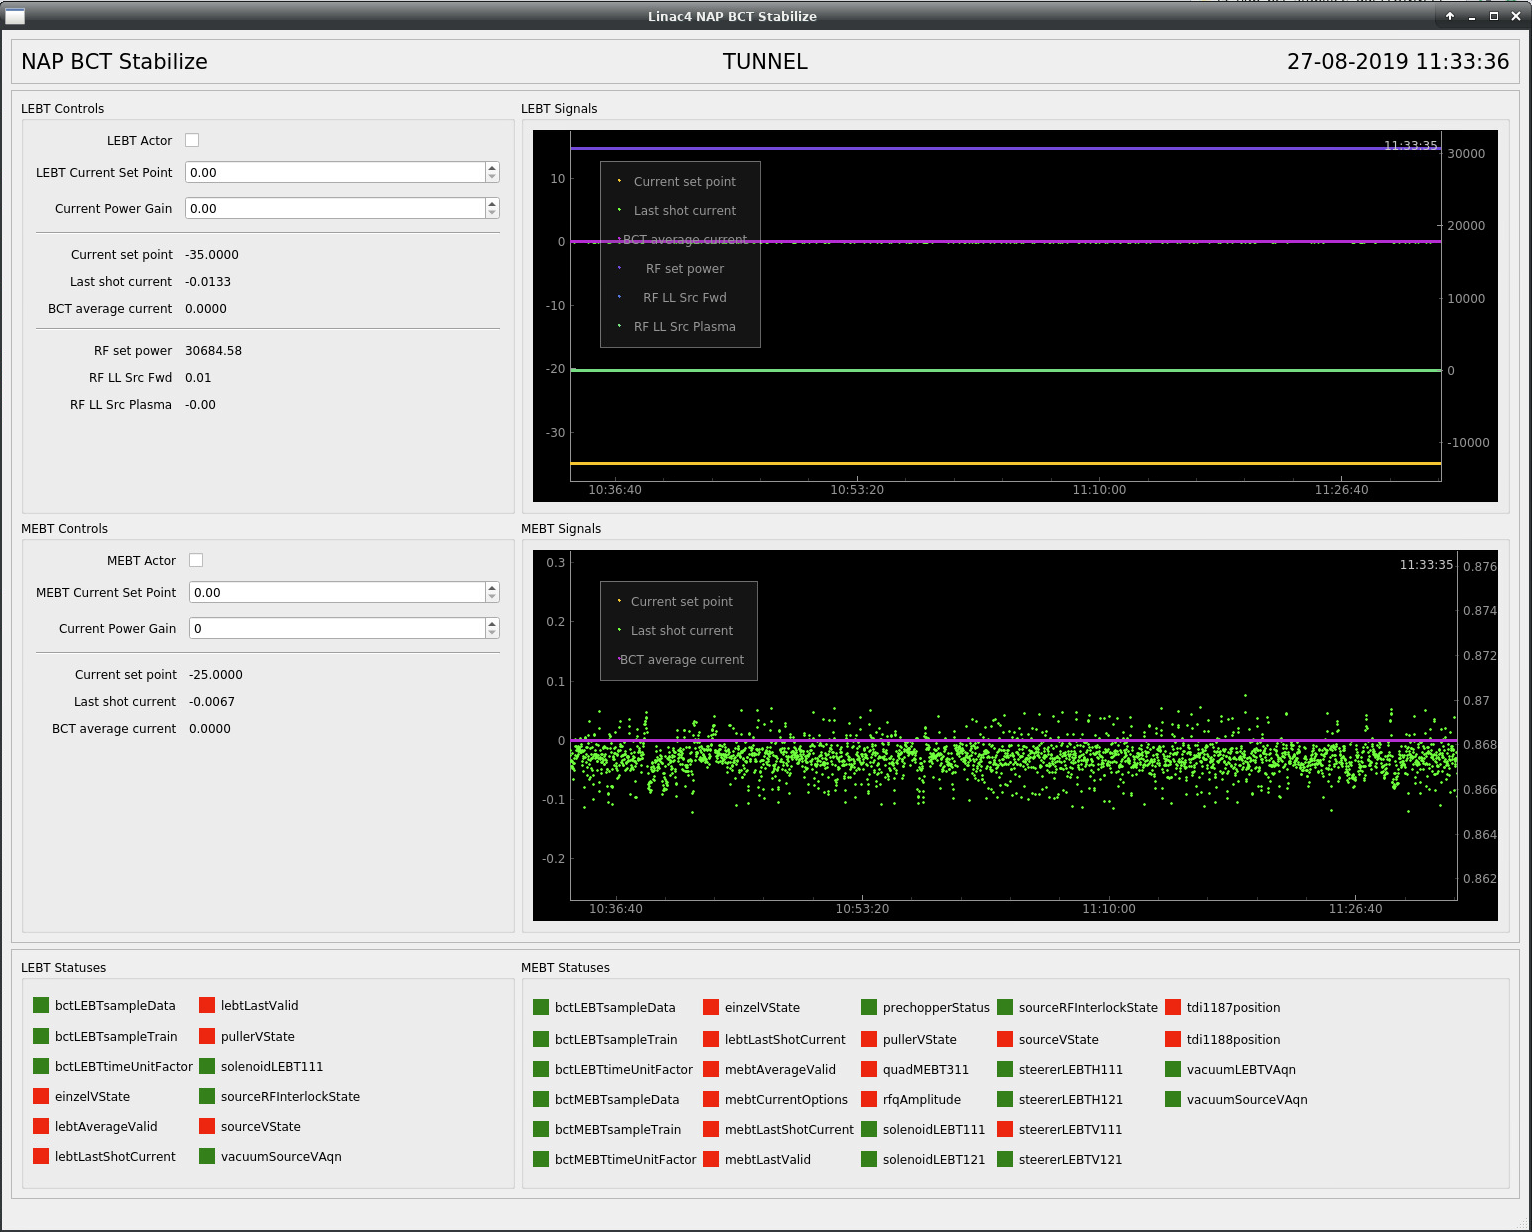
\includegraphics[width=14cm]{resources/img/Linac4SourceGui}
    \caption{Screenshot of the Linac4 Source Gui}
    \label{fig:linac4sourcegui}
\end{figure}

The Application where this Use Case is originated from is a \gls{gui} for the Linear Accelerator Linac4, whose tasks it is to boost negative hydrogen ions to high energies. The GUI will allow monitoring and manipulation of different device settings. Image \ref{fig:linac4sourcegui} shows a screenshot of an early version of the application. In the upper right part of the window are two graphs containing multiple scatter plots. Both graphs are implemented with the python graph library pyqtgraph, which we will explore in more detail in section \ref{sec:application:libraries:pyqtgraph}.
\cite{LinacFour,LinacFourGuiPres}


%% ==============================================
%%       Performance Metrics from Use Cases
%% ==============================================
\section{Performance Metrics from Use Cases}
\label{sec:usecases:metrics}

In this section we will collect metrics we can use to define a plotting libraries performance based on the insights we gained into the usage of these libraries from the use cases in this chapter. All of these Use Cases have in common, that they are displaying live data, which will be delivered with a certain frequency. If a plotting widget needs a very long time to redraw, this might result in updates piling up without the widget having time to redraw, if an update is always leading to a redraw. Long redraw cycles are not only a 
The most important metric we have to measure is without a doubt, how long the operations following a data update take. When collecting those times and calculating the average from it, we can make realistic predictions, if a widget will handle a certain update load under certain circumstances.

Even for applications containg graphs, which are not updated regularly, the time it takes the graph to redraw is very important for the interaction with the graphs, since it requires the graph to redraw as well. Slow redraw times will lead in these applications to stuttering use interfaces.

If a Use Case reveals a performance issue, it is important to investigate, where the source of the performance issue is rooted. Profiling is a very helpful procedure to decide, where improvements are needed most. A profile lists very detailed information about which functions consumed how much time in total, how often it has been called and how long a single call did take. With these informations, we can investigate, where we can change code to increase performance.
